% vim:foldmethod=marker:fmr=<<<,>>> spell nowrap
\documentclass{article}

% <<<
\usepackage[utf8]{inputenc}
\usepackage[total={6.2in, 8in}]{geometry}

\usepackage{amsmath, amsthm, amssymb,amsfonts, mathtools}
\usepackage{graphicx}
\usepackage{float}
\usepackage[percent]{overpic} %writing over pictures
\usepackage{xcolor}
\usepackage{appendix}

\usepackage{mdframed}
\usepackage[colorlinks,urlcolor=blue]{hyperref}
\usepackage{verbatim}
%\usepackage{fancyvrb}
\usepackage{minted}
\renewcommand{\MintedPygmentize}{pygmentize}
\usepackage[ruled,linesnumbered]{algorithm2e}
\setlength{\algomargin}{10pt}
\newcommand{\REM}[1]{\tcp*{\parbox[t]{2.0in}{\raggedright #1}}}
\usepackage[normalem]{ulem}
\usepackage{varwidth}

\usepackage{biblatex}
\addbibresource{main.bib}

\usepackage{listings}
\usepackage{tikz-cd}
\usepackage{enumitem}
\usepackage{tikzsymbols}

\lstset{
basicstyle=\small\ttfamily,
columns=flexible,
breaklines=true
}

\setlength{\parindent}{0pt}

\newcommand{\ket}[1]{\left|{#1}\right\rangle}
\newcommand{\bra}[1]{\left\langle{#1}\right|}
\newcommand{\BS}{\backslash}

\newcommand{\CLR}[2]{\begingroup\color{#1}#2\endgroup}
\newcommand{\R}[1]{\begingroup\color{red}#1\endgroup}
\newcommand{\G}[1]{\begingroup\color{green}#1\endgroup}
\newcommand{\B}[1]{\begingroup\color{blue}#1\endgroup}
\newcommand{\Y}[1]{\begingroup\color{yellow}#1\endgroup}
\newcommand{\N}{\mathbb{N}}
\newcommand{\Z}{\mathbb{Z}}
\newcommand{\Rational}{\mathbb{R}}
\newcommand{\Rat}{\mathbb{R}}

\newcommand{\vsp}[0]{\vspace*{10pt}\par}
\newcommand{\tcite}[1]{\textit{(\citefield{#1}{year}, \citeauthor{#1})}\:\textit{``\citefield{#1}{title}''}\:\cite{#1}}
\newcommand{\exercise}[1]{\subsubsection*{#1}}
\newcommand{\ans}[0]{\vsp\textbf{Answer: }\vsp}
\newcommand{\unsure}[0]{TODO: (\textbf{unsure}) }

\newcommand{\JProg}{\mathbb{J}}
\newcommand{\AST}{\mathbb{AST}}
\newcommand{\TNET}{\mathbb{TNET}}
\newcommand{\CV}{\Rational^N}

\newcommand{\ei}{\item}
\newcommand{\eb}{\begin{enumerate}[label=(\alph*)]\ei}
\newcommand{\ee}{\end{enumerate}}

% Define \set{} command. TODO: Looks too complicated!
\DeclarePairedDelimiterX{\set}[1]{\{}{\}}{\setargs{#1}}
\NewDocumentCommand{\setargs}{>{\SplitArgument{1}{;}}m}
{\setargsaux#1}
\NewDocumentCommand{\setargsaux}{mm}
{\IfNoValueTF{#2}{#1} {#1\,\delimsize|\,\mathopen{}#2}}%{#1\:;\:#2}

% Generic environment for code snippets
\newenvironment{codeverbatim}
  {\VerbatimEnvironment
   \begin{minted}[autogobble,breaklines,fontsize=\footnotesize]{latex}}
  {\end{minted}}
\BeforeBeginEnvironment{codeverbatim}{\begin{mdframed}[nobreak=true,frametitle=\tiny{Source}]}
\AfterEndEnvironment{codeverbatim}{\end{mdframed}}

% LitREPL-compatible environment for code snippets
\newenvironment{python}
  {\VerbatimEnvironment
   \begin{minted}[autogobble,breaklines,fontsize=\footnotesize]{python}}
  {\end{minted}}
\BeforeBeginEnvironment{python}{\begin{mdframed}[nobreak=true,frametitle=\tiny{IPython}]}
\AfterEndEnvironment{python}{\end{mdframed}}

% LitREPL-compatible environment for code results
\newenvironment{result}
  {\VerbatimEnvironment
   \begin{minted}[autogobble,breaklines,fontsize=\footnotesize]{text}}
  {\end{minted}}
\BeforeBeginEnvironment{result}{\begin{mdframed}[nobreak=true,frametitle=\tiny{Result}]}
\AfterEndEnvironment{result}{\end{mdframed}}

% LitREPL-compatible command for inline code results
\newcommand{\linline}[2]{#2}
\newcommand{\st}[1]{\sout{#1}}
\renewcommand{\t}[1]{\texttt{#1}}
% >>>

\setcounter{secnumdepth}{4}
% \RedeclareSectionCommand[runin=false,afterskip=0pt,afterindent=false]{paragraph}

\title{Category Theory for Scientists (Solutions)}
\author{Sergei Mironov}

\begin{document}

\maketitle

\tableofcontents

\section{Introduction}

The book \tcite{Spivak2013CategoryTF}.

\setcounter{section}{2}
\section*{Chapter 2. The Category of Sets}

\exercise{2.3.3.1}

Create an olog for human nuclear biological families that includes the concept of person, man,
woman, parent, father, mother, and child. Make sure to label all the arrows, and make sure each
arrow indicates a valid aspect in the sense of Section 2.3.2.1. Indicate with check-marks the
diagrams that are intended to commute. If the 2-dimensionality of the page prevents a check-mark
from being unambiguous, indicate the intended commutativity with an equation.

\ans

\begin{center}
% https://tikzcd.yichuanshen.de/#N4Igdg9gJgpgziAXAbVABwnAlgFyxMJZARgBoAGAXVJADcBDAGwFcYkQ0YAnOAkAX1LpMufIRTlSxanSat2AW3qFBw7Hj4oATFJkMWbRCADuEJSqEcRG8SVJa9cwx3pcYYHAMsZ1YopIBmRwN2ADN6HAALbi81UU1kHSCafXkjBQgomNUrXwSyABZgtJAAY0isRigBGRgoAHN4IlBQrjMkMhAcCCRJEEZ6ACMYRgAFaz8jRhhQzxSndiwEHNb2xB0unsQ+1OclkBoB4bGJzX6ZzxW2hSQCmm6O+ZCjfau1gFZ7rY3dxYRDoYjcZ5cQgLhYeqRS6WVY3RB3TZIAJPEqvGHXJCfRGIZGyZ4gfYA47A+Kg8GQ6EtDGILEPRAANnu9Eq7EgYDYKOckXo-36gJOIPY5KhsRAsNuXyQjLxJW5vKOQNOZIhIrecNxdOlvyMctF4pxku2nL+Bz5xKVQpVlLF1OldL6wzA1UQAFoAOydbUE+X8kk2S0U01wCqzJBafiUfhAA
\begin{tikzcd}
                                                            & person                                                  &                                                               \\
man \arrow[ru, "is"]                                        &                                                         & woman \arrow[lu, "is"]                                        \\
                                                            & parent \arrow[dd, "has"] \arrow[uu, "is"']              &                                                               \\
father \arrow[uu, "is"] \arrow[ru, "is"] \arrow[rd, "has"'] &                                                         & mother \arrow[uu, "is"'] \arrow[lu, "is"'] \arrow[ld, "has"'] \\
                                                            & child \arrow[uuuu, "is"', bend right=90, shift right=18] &
\end{tikzcd}
\end{center}

Commutative square examples:
\begin{itemize}
\item "parent is person" $\circ$ "mother is parent" $=$ "woman is person" $\circ$ "mother is woman"
\item "mother has child" $=$ "parent has child" $\circ$ "mother is parent"
\item "child is person" $\circ$ "parent has child" $\ne$ "parent is person"
\end{itemize}

\setcounter{subsection}{3}
\subsection{Products and coproducts}

\exercise{2.4.1.4}
How many elements does the $\set{a,b,c,d} * \set{1,2,3}$ have?
\ans
12

\exercise{2.4.1.8}
\ans
(a) No, because $a(b + c) \neq (a+b)c$.
\vsp
(b) No, because $x*0 \neq x$.
\vsp
(c) Yes.

\exercise{2.4.1.15}

(a) Let $X$ and $Y$ be sets.. construct the "swap map" $s:(X \times Y)\to(Y \times X)$
\ans
$s:(X \times Y)\to(Y \times X) = (,)\circ\langle\pi_2,\pi_1\rangle$

Note: we used angle brackets. Is it really correct?

\vsp
(b) Can you prove that $s$ is a isomorphism using only the universal property for product?

Note: $(f:X \to Y)$ is an isomorphism if $\exists (g:Y \to X): g \circ f = id_X \land f \circ g =
id_Y$

Note: diagram $(f,g,h)$ commutes if $f \circ g = h$
\ans

In universal property of products, put $A$ equal to $Y \times X$ and get $\exists !
g:(Y \times X)\to(X \times Y)$. In a similar way, we have $\exists! s:(X \times Y)\to(Y \times X)$.
We need to show that $g \circ s = id_{(X \times Y)}$ and $s \circ g = id_{(Y\times X)}$.

On the following diagram,

% https://tikzcd.yichuanshen.de/#N4Igdg9gJgpgziAXAbVABwnAlgFyxMJZARgBoAmAXVJADcBDAGwFcYkQBBAAgB0e8AtvC4AhEAF9S6TLnyEUZAAzU6TVu259BwsZOnY8BIuVLEVDFm0QhdUkBgNyii0+bVXOElTCgBzeESgAGYAThACSC4gOBBIZCCM9ABGMIwACjKG8iAhWL4AFjggNBbq1nwwAB5YcDhwAIRBEnah4ZE0MUgmqpbsfGhYAPrkxQnJqRmORta5BUV6IK0RiFGdiADMJe59PAODxM3BYcvxa5s9ZSD9Qwc0iSnpmU4zeYWHi8dxHbGI3aUe12GXnEQA
\begin{tikzcd}
  & A \times B \arrow[ld, "\pi_1"'] \arrow[rd, "\pi_2"]                           &   \\
A &                                                                               & B \\
  & A \times B \arrow[uu, "\exists!id"'] \arrow[ru, "\pi_2"'] \arrow[lu, "\pi_1"] &
\end{tikzcd}

$id = id_{(A \times B)}$ - is the unique identity function. By combining diagrams for $f$ and $g$ we
reduce the $g \circ f$ to the similar case.

\exercise{2.4.2.4}

Would you say that a phone is the coproduct of a \texttt{cellphone} and a \texttt{landline phone}?

\ans
Yes, until we consider other types of phones besides cell- and landline ones.

\exercise{2.4.2.10}

Write the universal property for coproduct in terms of a relationship between..

\ans \unsure $Hom_{Set}(X,A) \sqcup Hom_{Set}(Y,A) \cong Hom_{Set}(X \sqcup Y, A)$

\exercise{2.4.2.13}

TODO

\exercise{2.4.2.14}

TODO


\subsection{Finite limits in Set}

\exercise{2.5.1.2}

\ans $X \times_{Z} Y = \set{(x_1,z_1,y_1), (x_2,z_2,y_2), (x_2,z_2,y_4), (x_3,z_2,y_2),
(x_3,z_2,y_4)}$


\exercise{2.5.1.3}

(a)
\ans Let $X = \set{\Y{1},\R{2},\B{3},\Y{4},\R{5}}; Y = \set{\Y{a},\B{b},\R{c}};$ where
$C = \set{\R{R},\B{B},\Y{Y}}$ \vsp We have:
$X \times_C Y = \set{\Y{1a},\Y{4a},\R{2c},\R{5c},\B{3b}}$

(b)
TODO (obvious).

\exercise{2.5.1.5}

(a) Suppose that $Y = \emptyset$; what can you say about $X \times_Z Y$ ?
\ans $X \times_Z Y = \emptyset$ \vsp

(b) $Z = {1}$; what can you say about $X \times_Z Y$ ?
\ans $\forall X,Y : X \times_Z Y \cong X \times Y$

\exercise{2.5.1.6}

.. Aristotelian space and time ..

$S = R^3;\quad T = R;\quad Y = S \times T;\quad g1 : Y \to S ;\quad g2 : Y \to S$ where $g1,g2$
projects space-time to its components. $X = \set{1};\quad f_1 : X \to S;\quad f_2 : X \to T$ is a
set of one element and its space-time projections.

\vsp
(a) What is the meaning of

\begin{minipage}[t]{0.45\textwidth}
\[
\begin{tikzcd}
W_1 \arrow[r] \arrow[d] & Y \arrow[d,"g_1"] \\
X \arrow[r,"f_2"] & S
\end{tikzcd}
\]
\end{minipage}
\quad
\begin{minipage}[t]{0.45\textwidth}
\[
\begin{tikzcd}
W_2 \arrow[r] \arrow[d] & Y \arrow[d,"g_2"] \\
X \arrow[r,"f_2"] & S
\end{tikzcd}
\]
\end{minipage}

\ans $1$ is associated with its time and space. $W_1$ yields time points of $Y$ corresponding
to $1$'s position. $W_2$ yields the space points corresponding to $1$'s time.

\vsp
(b) Interpret the sets in terms of the center of mass of MIT at the time of its founding.

\ans \unsure Is it just the MIT-relative space and time points?

\exercise{2.5.1.10}

.. Appropriate or misleading olog labels ..

\ans
(a) a person whose favorite color is blue - OK
\vsp
(b) a dog whose owner is a woman - OK
\vsp
(c) a good fit - Nope. We would say that a good fit requires less or equal width.

\exercise{2.5.1.11}

(a) Consider your olog from Exercise 2.3.3.1. Are any of the commutative
squares there actually pullback squares?

\ans
Yes, for example: "father" $=$ "man" $\times_{person}$ "parent"

\begin{center}
\begin{tikzcd}
\fbox{father} \arrow[r, "is"] \arrow[d, "is"] & \fbox{man} \arrow[d,"is"] \\
\fbox{parent} \arrow[r,"is"]                  & \fbox{person}
\end{tikzcd}
\end{center}

(b) Now use ologs with products and pullbacks to define what a brother is and
what a sister is:

\ans

\begin{center}
% https://tikzcd.yichuanshen.de/#N4Igdg9gJgpgziAXAbVABwnAlgFyxMJZABgBpiBdUkANwEMAbAVxiRACMAnCHACxk4gAvqXSZc+QigCM5KrUYs2AY15YGUYaJAZseAkTLT59Zq0QgAtnUIixeyUVnHqppRYyWt9iQZmkAJhNFcx0BOAM7HXF9KWQA0hcFMzYAHVTgABV0oW9ohz94wOCUi3Ss0gAxHOF5GCgAc3giUAAzbi9EAGZqHAgkABZXELTUtCwAfWk89ohOnpA+pABWYdKQdPGJgJmOld7+xAA2NfcQLE0o2c6hxcOT5LOwCeBVXKu9xDI7pFlH0KwCA+cyQ3yWiAS-zYgN2IIhByQCzcoTQsM6f3BSJGHlqQiAA
\begin{tikzcd}
brother \arrow[r, "is"] \arrow[d, "is"] & child \arrow[d, "p"]                      &                       \\
man \arrow[r, "p"]                      & pom \arrow[d, "\pi_1"] \arrow[r, "\pi_2"] & \{T\} \arrow[d, "id"] \\
                                        & person \arrow[r, "n_{ch}"]                & {\{T,F\}}
\end{tikzcd}
\end{center}

where: $pom$ stands for "parent of many", $p$ is "has as parent" and $n_{ch}$
is "number of children"

\exercise{2.5.1.13}

Pullback diagram in which the fiber product is isomorphic to the preimage of $y \in Y$.

\ans

\begin{center}
% https://tikzcd.yichuanshen.de/#N4Igdg9gJgpgziAXAbVABwnAlgFyxMJZABgBpiBdUkANwEMAbAVxiRAE0A9YAWgEYAvgB0heALbwABHwD6ATxADS6TLnyEUfclVqMWbWQqUrseAkTJ8d9Zq0QgAGouUgMp9US1XqN-ffaKOjBQAObwRKAAZgBOEGJIWiA4EEgAzD56diBYUM5RsfGIAEzUyWkZtmyReSAxcUhkSSmIib5ZImhYMkU1dYWNZcUVfiAdXXyBAkA
\begin{tikzcd}
Y^{-1} \times \set{y} \arrow[r, "\pi_2"] \arrow[d, "\pi_1"] & \set{y} \arrow[d, "id"] \\
X \arrow[r, "f"]                                            & Y
\end{tikzcd}
\end{center}

\exercise{2.5.1.15}

Create an olog whose underlying shape is a commutative square. Now add the
fiber product so that the shape is the same as that of Diagram (2.32). Assign
English labels to the projections and to the dotted map A, such that these
labels are as canonical as possible.

\ans

\unsure

The general impression is the following:
\begin{itemize}
  \item The commutative square can be visualized as a pyramid in a 3D space.
  \item The pullback corresponds to a 2D plane with two axes.
  \item The pullback over one-element set corresponds to a 2D plane with two orthogonal axes.
  \item The projections $\pi_1$ and $\pi_2$ play the role of parallel
        projections from a point in the plane to its axes.
  \item The map $A \to (D \times_P W)$ acts as a projection from a point in 3D space to the plane.
\end{itemize}

\begin{center}
% https://tikzcd.yichuanshen.de/#N4Igdg9gJgpgziAXAbVABwnAlgFyxMJZARgBpiBdUkANwEMAbAVxiRAAUB1AEQHkQAvqXSZc+QigAMpAExVajFm26DhIDNjwEiM2fPrNWiEJ1UjN4omQDM+xUY4wATnG1DzY7SjKS7htjz8AvIwUADm8ESgAGZOEAC2SAAs1DgQSGQgAEYwYFBIALTW0gr+xgA65WhYAPrEZiCxCcmp6Yi62bn5iMXUBkoVVbUyINQMdDkM7KJaEiBOWGEAFjgNTYmImWlI1u6NcRsd2z1760glx5n9DtUAxjX5pwfnrUgd45PTFl7ziyujpQG6iw92AAHcBGtnogLm0UoCbiCasA0HQsE5IcEBEA
\begin{tikzcd}
             & \fbox{($D \times_P W$) \text{woman dog owner}} \arrow[ldd, "\pi_1", bend right] \arrow[rdd, "\pi_2"', bend left]        &              \\
             & \fbox{(A)\begin{varwidth}{\textwidth} blond woman \\ dog owner \end{varwidth}} \arrow[ld, "has"] \arrow[rd, "is"'] \arrow[u, "\langle\text{has, is} \rangle"] &              \\
\fbox{(D) dog} \arrow[rd] &                                                                                        & \fbox{(W) woman} \arrow[ld] \\
             & \fbox{(P) person}                                                                                   &
\end{tikzcd}
\end{center}

\exercise{2.5.1.18}

(a) Create an olog that defines two people to be 'of approximately the same
height' if and only if their height difference is less than half an inch, using
a pullback.

\ans

\begin{center}
% https://tikzcd.yichuanshen.de/#N4Igdg9gJgpgziAXAbVABwnAlgFyxMJZABgBpiBdUkANwEMAbAVxiRAEEQBfU9TXfIRRkAjFVqMWbAELdeIDNjwEiI8uPrNWiEAGE5fJYNWkx1TVJ0ARAwv7KhyAEzrzk7SACitxQJUoXMwktNgAxbnEYKABzeCJQADMAJwgAWyQyEBwIJCceRJT0xBcsnMQAFnyQZLSkcupspABWKpqigGYGspb5NqQ1UqR21sLcrqGR2sRMxsQRLgouIA
\begin{tikzcd}
  \set{((p_1,p_2),\Delta)|p_1,p_2 \in \text{people}, \Delta \in \Rational} \arrow[r, "\pi_2"] \arrow[d, "\pi_1"] & \set{\Delta|-0.5 < \Delta < 0.5} \arrow[d, "is"] \\
  \fbox{\text{pair of people}} \arrow[r, "h_2 - h_1"]           & \Rational
\end{tikzcd}
\end{center}

(b) In the same olog, make a box for those people whose height is approximately
the same as a person named 'The Virgin Mary'. You may need to use images.

\ans

\begin{center}
% https://tikzcd.yichuanshen.de/#N4Igdg9gJgpgziAXAbVABwnAlgFyxMJZABgBpiBdUkANwEMAbAVxiRAEEQBfU9TXfIRRkAjFVqMWbAELdeIDNjwEiI8uPrNWiEAGE5fJYNWkx1TVJ0ARAwv7KhyAEzrzk7SACitxQJUoXMwktNgAxbnEYKABzeCJQADMAJwgAWyQyEBwIJCceRJT0xBcsnMQAFnyQZLSkcupspABWKpqigGYGspb5NqQ1UqR21sLcrqGR2sRMxsQRLgouIA
\begin{tikzcd}
  \fbox{\text{people of approx Virgin Mary height}} \ar[r, "\pi_2"] \ar[d, "\pi_1"] & \set{((p_1,p_2),\Delta)|...} \arrow[r, "\pi_2"] \arrow[d, "\pi_1"] & \set{\Delta|-0.5 < \Delta < 0.5} \arrow[d, "is"] \\
  \set{(\fbox{The Virgin Mary},p_2)|p_2 \in \text{people}} \ar[r, "is"] & \fbox{\text{pair of people}} \arrow[r, "h_2 - h_1"]           & \Rational
\end{tikzcd}
\end{center}

\unsure We did not use images, despite the textbook suggestion.

\exercise{2.5.1.19}

Let $W = X \times_Z Y$ and $W' = X' \times_{Z'} Y'$, and form the diagram
to the right. Use the universal property of fiber products to construct a map
$W \to W'$ such that all squares commute

\ans

Let $WX = \pi_1$, $WY = \pi_2$, $W'X' = \pi_1'$, $W'Y' = \pi_2'$.  Define $f: W
\to W' = (x,y)_z \mapsto (XX'(x),YY'(y))_{ZZ'(z)}$. We want to show that it
makes $WW'Y'Y$ to commute. Indeed, $\pi_2' \circ f = YY' \circ \pi_2 = y
\mapsto YY'(y)$.  By analogy, it also commutes $WW'X'X$. The triangles $WW'Y'$
and $WW'X'$ also commute. The universal property for fiber products says that
we can only have one such mapping, thus this is the answer.


\exercise{2.5.2.6}

(a)
TODO: Copy the picture from the book notes

(b)
TODO: Copy the picture from the book notes

(c)
TODO: Find the correct answer


\exercise{2.5.3.3}

Come up with an olog that uses equalizers in a reasonably interesting way.
Alternatively, use an equalizer to specify those published authors who have
published exactly one paper. Hint: find a function from authors to papers; then
find another.

\ans

We follow the second way.

\begin{center}
\begin{tikzcd}[column sep=3cm]
\text{Authors} \arrow[r, "\text{num of papers}", "\text{const}_1"', Rightarrow] & \Rational
\end{tikzcd}
\end{center}

where $const_1 : \text{authors} \to \Rational$ maps all authors to $1$.

\exercise{2.5.3.4}

Find a universal property enjoyed by the equalizer of two arrows, and present
it in the style of Lemmas 2.4.1.10, 2.4.2.7, and 2.5.1.14.

\ans

For any set $A$, function $f$ and $g$ there exists unique $u$ mapping $A$ to
$Eq(f,g)$ such that everything commute, in particular, $\pi \circ u = p$.

\begin{center}
% https://tikzcd.yichuanshen.de/#N4Igdg9gJgpgziAXAbVABwnAlgFyxMJZABgBoBmAXVJADcBDAGwFcYkQBNEAX1PU1z5CKMgCZqdJq3YANHnxAZseAkTIBGCQxZtEIAILz+yoWtLEtU3SACiARwAUAM1IBzAJQ8JMKK-hFQJwAnCABbJFEaHAgkcl5AkPDESJBopHV4kGCw9KiYxDIQRiwwaygIZgAjRjYaAAsYeigkMGZGRij6LEZ2SFKjLMTYvNyQSpgwZsQAWgA2AHZuSm4gA
\begin{tikzcd}
{Eq(f,g)} \arrow[dd, "\pi", bend right=67]      \\
A \arrow[u, dashed, "\exists!u"] \arrow[d, "p"] \\
X \arrow[d, Rightarrow, "g", "f"']              \\
Y
\end{tikzcd}
\end{center}

\exercise{2.5.3.5}

(a) A terminal set is a set $S$ such that for every set $X$, there exists a
unique function $X \to S$. Find a terminal set.

\ans

Any set $S$ with one element. There exist exactly one function $X \to S$ so it
is unique.

\vsp

(b) Do you think that the notion \textit{terminal set} belongs in this section (Section
2.5)? How so?  If products, pullbacks, and equalizers are all limits, what do
limits have in common?

\ans

A terminal set $S$ is terminal because it has canonical projections
(inclusions) back to $X$ (and $Y$, if applicable). We suppose that the way they
work does not change from category to category.


\subsection{Finite colimits in Set}

\exercise{2.6.1.3}

Let $X$ be the set of people on earth; define a binary relation $R \subseteq (X
\times X)$ on $X$ as follows. For a pair $(x, y)$ of people, say $(x, y) \in R$
if $x$ spends a lot of time thinking about $y$.
\ans
(a) Is this relation reflexive? No.

(b) Is it symmetric? No.

(c) Is it transitive? No.

\exercise{2.6.1.5}

Take a set $I$ of sets; i.e. suppose that for each element $i \in I$ you are
given a set $X_i$. For every two elements $i,j \in I$ say that $i \sim j$ if
$X_i$ and $X_j$ are isomorphic. Is this relation an equivalence relation on
$I$?

\ans

Any set is isomorphic to itself, so $\sim$ is reflexive; isomorphism is also
symmetric and transitive. So, yes, $\sim$ is an equivalence relation.

\exercise{2.6.1.9}

Consider the set R of real numbers. Draw the coordinate plane $\Rational
\times \Rational$, give it coordinates $x$ and $y$. A binary relation on
$\Rational$ is a subset $S \subseteq \Rational \times \Rational$, which can
be drawn as a set of points in the plane.

\vsp

(a) Draw the relation $\set{(x,y)|y=x^2}$.

(b) Draw the relation $\set{(x,y)|y \ge x^2}$.

(c) Let $S_0$ be the equivalence relation on $R$ generated (in the sense of
Lemma 2.6.1.7) by the empty set. Draw $S$ as a subset of the plane.

(d) Consider the equivalence relation $S_1$ generated by $\set{(1,2),(1,3)}$.
Draw $S_1$ in the plane. Highlight the equivalence class containing $(1,2)$.

(e) The reflexivity property and the symmetry property have pleasing
visualizations in $\Rational \times \Rational$; what are they?

(f) Is there a nice heuristic for visualizing the transitivity property?

\ans

\begin{comment}
\begin{python}
import matplotlib.pyplot as plt
import numpy as np
D = 3
x = np.linspace(-D, D, 100)
y = x**2
plt.close('all')
plt.figure()
plt.plot(x, y)
plt.fill_between(x, y, max(y), where=(y > 0), color='none', hatch='/', edgecolor='b', linewidth=0.5)
plt.xlabel('x')
plt.ylabel('y')
plt.xticks(np.arange(-D, D+1, 1))          # Set x-axis to cover integer values
plt.yticks(np.arange(-2, max(y) + 1, 1))    # Set y-axis to cover integer values
plt.grid(True)
plt.title('Parabola: y = x^2')
plt.grid(True)
for ix in range(-D, D+1):
  for iy in range(-2, D**2+1):
    if 1<=ix<=3 and 1<=iy<=3:
      plt.plot(ix, iy, 'bo')  # 'ro' defines red dots
    if ix==iy:
      plt.plot(ix, iy, 'ro')  # 'ro' defines red dots

plt.savefig('img/parabola.png')
\end{python}
\begin{result}
\end{result}
\end{comment}

\begin{center}
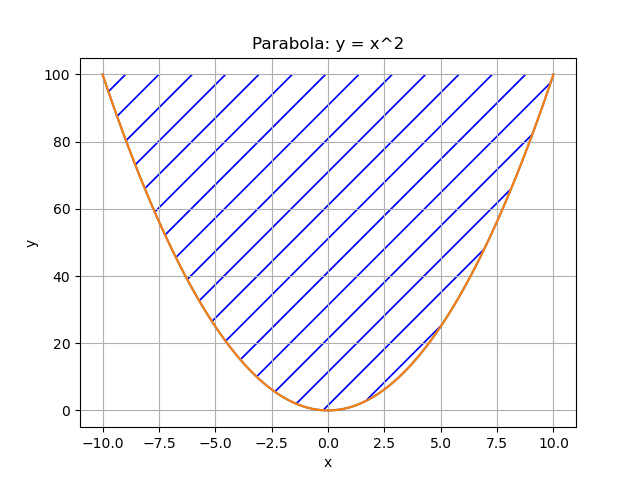
\includegraphics[width=0.4\textwidth]{img/parabola.png}
\end{center}

\eb the line
\ei the filled area
\ei red dots
\ei square of blue dots, including the diagonal
\ei The representation of a reflexivity relation in rational numbers is the diagonal line on a 2D
    plane. The representation of a symmetry of a set on a 2D plane is the set itself and its mirror
    image across the diagonal
\ei TODO: Something like this?
    \begin{center}
    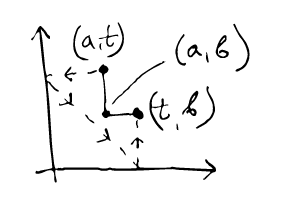
\includegraphics[width=0.3\textwidth]{img/heuristic.png}
    \end{center}
\ee

\exercise{2.6.1.10}

Consider the binary relation $R = \set{(n,n+1)|n\in\Z}\subseteq\Z\times\Z$.

\eb What is the equivalence relation generated by $R$?
\ei How many equivalence classes are there?
\ee

\ans

\eb Whole $\Z$.
\ei One.
\ee

\exercise{2.6.1.11}

Suppose $N$ is a network (or graph). Let $X$ be the nodes of the network, and
let $R \subseteq X \times X$ denote the relation such that $(x, y) \in R$ iff
there exists an arrow connecting $x$ to $y$.

\eb What is the equivalence relation $\sim$ generated by $R$?
\ei What is the quotient $X/\sim$?
\ee

\ans

\eb For each disjoint subgraph $g \subseteq N$, the relation $R$ represents a
    fully connected graph $g'$ formed by the vertices of $g$.
\ei A set of disjoint graphs.
\ee

\exercise{2.6.2.4}

(The picture) Write down the cardinality of $P \cong \underline{n}$ as a natural
number $n \in \N$.

\ans

$1$, because the described $W \to X$ and $W \to Y$ make all elements of $X$ and
$Y$ equivalent.

\exercise{2.6.2.5}

Suppose that $W = \emptyset$; what can you say about $X \sqcup_W Z$?

\ans

$X \sqcup_W Z$ becomes $X \sqcup Z$ because $(X \sqcup W \sqcup Z)/\sim$ is
filled with distinct elements of both $X$ and $Z$.

\exercise{2.6.2.6}

Let $W := \N = \set{0,1,2,... }$ denote the set of natural numbers, let $X =
\mathbb{Z}$ denote the set of integers, and let $Y = \set{\Smiley}$ denote a
one-element set. Define $f : W \to X$ by $f(w) = -(w+1)$, and define $g: W \to Y$ to be
the unique map. Describe the set $X \sqcup_W Y$ .

\ans

$X \sqcup_W Y = \set{\Laughey, 1, 2, 3}$ where $\Laughey$ is equivalent to all
the items of $\set{..., -2, -1, 0, \Laughey}$.

\exercise{2.6.2.7}

Let $i: R \subseteq X \times X$ be an equivalence relation. Composing with the
projections $\pi_1, \pi_2 : X \times X \to X$, we have two maps $\pi_1 \circ i :
R \to X$ and $\pi_2 \circ i: R \to X$.

\eb What is the pushout $X - R - X$
\ei If $i: R \subseteq X \times X$ is not assumed to be an equivalence relation,
    we can still define the pushout above. Is there a relationship between the
    pushout $X - R - X$ and the equivalence relation generated by $R \subseteq X
    \times X$
\ee

\ans

\eb For any equivalence class in $R$, the pushout $X \sqcup_{i} X$ merges all
    the points belonging to it into a single element.
\ei If $i' : R' \subseteq X \times X$ is not an equivalence relation, then its
    pushout $|X \sqcup_{i'} X| > |R|$ where $R$ is the equivalence relation
    generated by $R'$.
\ee

\exercise{2.6.3.2}

Let $X = R$ be the set of real numbers. What is the coequalizer of the two maps
$X \to X$ given by $f = x \mapsto x$ and $g = x \mapsto (x + 1)$ respectively?

\ans

The coequalizer $Coeq(f,g) \sim [0,1) \subset \Rat$.

\exercise{2.6.3.3}

Find a universal property enjoyed by the coequalizer of two arrows.

\ans

For any set $A$, function $f$ and $g$, there exists unique $u$ mapping $A$ to
$Coeq(f,g)$ such that everything commute, in particular, $u \circ i = q$.

\begin{center}
% https://tikzcd.yichuanshen.de/#N4Igdg9gJgpgziAXAbVABwnAlgFyxMJZABgBoBmAXVJADcBDAGwFcYkQBhCGARwAoAZqQDmAShABfUuky58hFGQBM1Ok1bsAgpOkgM2PASJkAjKoYs2iEAE0dMg-OOli59VZAANSaphRh8ESgAgBOEAC2SGQgOBBIJjSMWGAeUPRwABZ+9iChEUjkNLFISonJqRDMAEaMbDRZ9FBIYMyMjEX0WIzskCk5eZGIpTFxiCZSwWGDw8WI0VUwYE2IAGwA7BKUEkA
\begin{tikzcd}
X \arrow[d, Rightarrow, "g", "f"']             \\
Y \arrow[d, "q"] \arrow[dd, bend left=67, "i"] \\
A                                              \\
{Coeq(f,g)} \arrow[u, dashed, "\exists!u"]
\end{tikzcd}
\end{center}


\exercise{2.6.3.4}

(Initial object). An initial set is a set S such that for every set A, there
exists a unique function $S \to A$

\eb Find an initial set
\ei Do you think that the notion initial set belongs in this section (Section
    2.6)? How so? If coproducts, pushouts, and coequalizers are all colimits,
    what do colimits have in common?
\ee

\ans

\eb Initial object for sets is the empty set.
\ei Colimits are isomorphic up to the unique isomorphism (???)
\ee

\subsection{Other notions in Set}

\exercise{2.7.1.2}

Create an olog that includes sets $X$ and $Y$ , and functions $f : X \to Y$ and
$g: Y \to X$ such that $g \circ f = id_X$ but such that $f \circ g \ne id_Y$;
that is, such that $f$ is a retract section but not an isomorphism.

\ans

TODO

\exercise{2.7.2.2}

For a finite set $A$, let $|A| \in \N$ denote the cardinality of (number of
elements in) $A$. If $A$ and $B$ are both finite (including the possibility that
one or both are empty), is it always true that $|B^A| = |B|^{|A|}$?

\ans

TODO

\exercise{2.7.2.4}

Let $X = \set{1, 2}$, $A = \set{a, b}$, and $Y = \set{x, y}$

\eb Write down three distinct elements of $L := Hom_{Set}(X \times A, Y)$
\ei Write down all the elements of $M := Hom_{Set}(A, Y)$
\ei For each of the three elements $l \in L$ you chose in part (a), write down
    the corresponding function $\phi(l): X \to M$ guaranteed by Proposition
    2.7.2.3.
\ee


\exercise{2.7.2.5}

Let $A$ and $B$ be sets.  We know that $Hom_{Set}(A, B) = B^A$, so we have a
function $id_{B^A} : Hom_{Set}(A, B) \to B^A$. Look at Proposition 2.7.2.3,
making the substitutions $X = Hom_{Set}(A, B)$, $Y = B$, and $A = A$. Consider
the function

\vsp

$\phi^{-1} : Hom{Set}(Hom_{Set}(A, B), B^A) \to Hom_{Set}(Hom_{Set}(A, B) \times A, B)$

\vsp

obtained as the inverse of (2.42).  We have a canonical element $id_{B^A}$ in
the domain of $\phi^{-1}$.  We can apply the function $\phi^{-1}$ and obtain an
element $ev = \phi^{-1}(id_{B^A}) \in Hom_{Set}(Hom_{Set}(A, B) \times A, B)$,
which is itself a function:

\vsp
$ev: Hom_{Set}(A, B) \times A \to B$
\vsp

\eb Describe the function $ev$ in terms of how it operates on elements in its domain.
\ei Why might one be tempted to denote this function by $ev$?
\ee

\ans

TODO

\exercise{2.7.2.6}

In Example 2.4.1.7 we said that $\Rational^2$ is an abbreviation for $\Rational
\times \Rational$, but in (2.43) we say that $\Rational^2$ is an abbreviation
for $\Rational^{\underline{2}}$. Use Exercise 2.1.2.14, Proposition 2.7.2.3,
Exercise 2.4.2.10, and the fact that $1+1=2$, to prove that these are
isomorphic, $\Rational^2 = \Rational \times \Rational$

\ans

TODO

\vsp
\vsp
\vsp
\vsp

\printbibliography

\end{document}

